% Please do not change the document class
\documentclass{scrartcl}

% Please do not change these packages
\usepackage[hidelinks]{hyperref}
\usepackage[none]{hyphenat}
\usepackage{setspace}
\doublespace

% You may add additional packages here
\usepackage{amsmath}
\usepackage{graphicx}

% Please include a clear, concise, and descriptive title
\title{Using Falmouth Adversity to better myself}

% Please do not change the subtitle
\subtitle{COMP150 - CPD Report}

% Please put your student number in the author field
\author{1707981}

\begin{document}

\maketitle

\section{Introduction} % 95 words
I meant University.

One day, I want to create a company around an initial game prototype, and play a creative lead role in its final production. Bringing my prototypes to life is my goal during this course, and if I can become so confident, to build a team around one of them.

First, I need to put my work where my mouth is. Then I must put my mouth out there. Here lie skills I must learn to do that, along with fragments of the better person to climb out of all this. Like a zombie.

\section{Skills to improve}
\subsection{Affective - Social Anxiety and Reaching Out} % 197 words
In the professional industry, it is virtually impossible to be noticed when hidden in a closet (unless that closet is in an inappropriate location, such as an airport runway). Making contacts is necessary for finding work, so avoiding people is counter to making a mark as an industry leader.

I delay tasks that involve initiating contact with people, despite wanting more. Ordering my DSA laptop in October was one example: this required a few phone calls; ultimately, I completed the process by January. My anxiety changes my priorities despite the positive investment, such as the ability to study anywhere. Sometimes I'll instead be `productive' by working on assignments. Since it's more comfortable to overwork than to pick up a phone, my anxiety is regularly mistaken for masochism.

I will read `The Shyness \& Social Anxiety Workbook' \cite{autismsucks} by M. Antony and R. Swinson. It challenges social anxiety through proven psychological techniques. For at least five days per week, in the evenings before I sleep, I'll read at least six pages, aiming to acknowledge and reduce my avoidance habits. My current goal is to finish the book at this pace or faster, whilst employing any of its advice where comfortable.

\subsection{Interpersonal - Being Inspirational} % 193 words

I believe sharing exciting collaborative ideas is symbolic of a good indie team. Unavoidably, the creative lead position requires the ability to coordinate differing ideas.

During Unreal project meetings, few people expressed ideas, possibly for fear of impacting someone else's, or otherwise sparking conflict. As one who is often shy to speak out amongst differing ideas, I question whether there are no ideas, or if everyone's just suppressing them. We need inspiration either way, and I currently lack the charisma to inspire them with words.

But I want to spark their motivation, and demonstrate a possible creative vision at the same time. So before February, I'll compose four short music pieces for the Unreal game using LMMS. I'll make a new short theme proposal every Sunday from the 7th Jan until the 28th, fifteen seconds minimum, completing any that I like in my own time. I'll pitch them all in the following meeting.

I believe a great project is one that creatives enjoy working on, even in their free time. Hopefully by setting an example, they'll become more interested in putting their creations forward too, regardless of my charisma or quality of work.

\subsection{Dispositional - Multi-tasking} % 203 words (oh dear)

Throughout the semester, my assignments took precedence over challenging real-life domestic tasks. I tend to focus on the goals of others. When I had time to work on my Arduino project or the group game project, I focused heavily on completing the latter. This was driven partly by a fear of submitting an incomplete-seeming game where the mark was shared across my team.

Judging by my actions, my motivation mostly comes from the expectation of meeting specific criteria--and I prefer letting others define it. When a criteria is vague, I lose motivation to meet them as i can't tell when it'll be done. Social anxiety can worsen the impact. 

To occupy myself over the summer, I aim to find a programming internship position somewhere in Brighton--another challenging prospect, that could benefit from being given specific criteria. This time using the LifeRPG app to track my progress, and maybe gaining motivation using its exp reward system, I will a) add my projects, music, artwork, and CV to my website, by Sunday 6/5/2018; b) update my LinkedIn profile by Wednesday 9/5/2018; and c) prospectively email 3 companies by Sunday 13/5/18.

\subsection{Cognitive - Class Shenanigans and Instantiation} % 203 words (oh dear oh dear)

It was Week 5. In our Object class, I created a `collision' attribute, declaring it as a default-initialised CollisionParams object. However, I quickly noticed that object instances were all sharing the same, modifiable CollisionParams object! Furthermore, if I initialised it in Object.\_\_init\_\_ instead, inherited classes wouldn't create it.

So I made `collision' optional, with my code ignoring it if it was None. My rationale was that if a programmer forgot to initialise it, their mistake would be obvious. However, my `solution' added bloating due to the if-statements. Retrospectively, the parent class should be initialised fully by every child class, using super().\_\_init\_\_(). I overlooked that, assuming it cumbersome, to the irony of the if-statements' wrath.

Since I resolved that already, my new learning goal is slightly different, but related to similar practices. In the past, I avoided C++ virtual functions, because I avoided the new operator: it would conflict with my fast allocation tools. However, I recently embraced \textit{new overloading}, making the switch possible. So in my upcoming C++ coursework, I'll instantiate all my dynamically-allocated classes with some form of `new', and I'll use virtual functions for inheritance. I'll tackle new, unfamiliar obstacles as they come, using my diary to record solutions.

\subsection{Procedural - It's not Broken until It's Made (Prototyping)} % 190 words (what a save!)

During comp150, I wrote the collision system for Frontier. I obsessed over its precision, for two reasons: one, to exercise a full understanding of the math behind it; and two, I like precision. I'm happy with both; however, in a prototyping scenario, this is not necessary. I neglected the greater context: we just needed a functional demo. Only after Michael's advice did I stop obsessing and finally prototype it with XY-aligned bounding boxes. This imperfection burnt my soul, but enabled me to work sooner on demonstrable mechanics that made the game look better in a shorter time. 

This is still a regular habit of mine. So next time, when taking a user story, I'll create a checklist of tasks to achieve the \textit{literal} user story. This addresses \textbf{no details} beyond the user story provided; for example, 'I want to fight an enemy' would provide the ability to attack an enemy, but the enemy won't attack back. Additional features must not yet be made. To enforce this, I'll create an `Optional' checklist on each user story I take, where I'll suggest precision and features which could be explored in leftover time.

\section{Recording Progress with the Diary} % 20 words

For some domains, I will measure progress with a weekly Google Docs diary, planned each Monday. See Appendix - Diary Template.

\section{Conclusion} % 93 words

I have ambitious life goals, but regardless of whether I reach them, improving these skills will help me find my place in industry. The first step to managing approach anxiety is being aware of proven techniques, hence the book. To avoid overload, I'm taking a creative approach to the interpersonal domain rather than socially-oriented. For the dispositional domain, I'll force multi-tasking through scheduled practice. Cognitively, awareness of standard class constructs is necessary in professional C++. Finally, there will be stalls during production, which I will reduce with a minimalistic approach to user stories.

\bibliographystyle{ieeetran}
\bibliography{references}

\newpage
\section{Appendix - Diary Template}
\begin{figure}[h]
\centering
\fbox{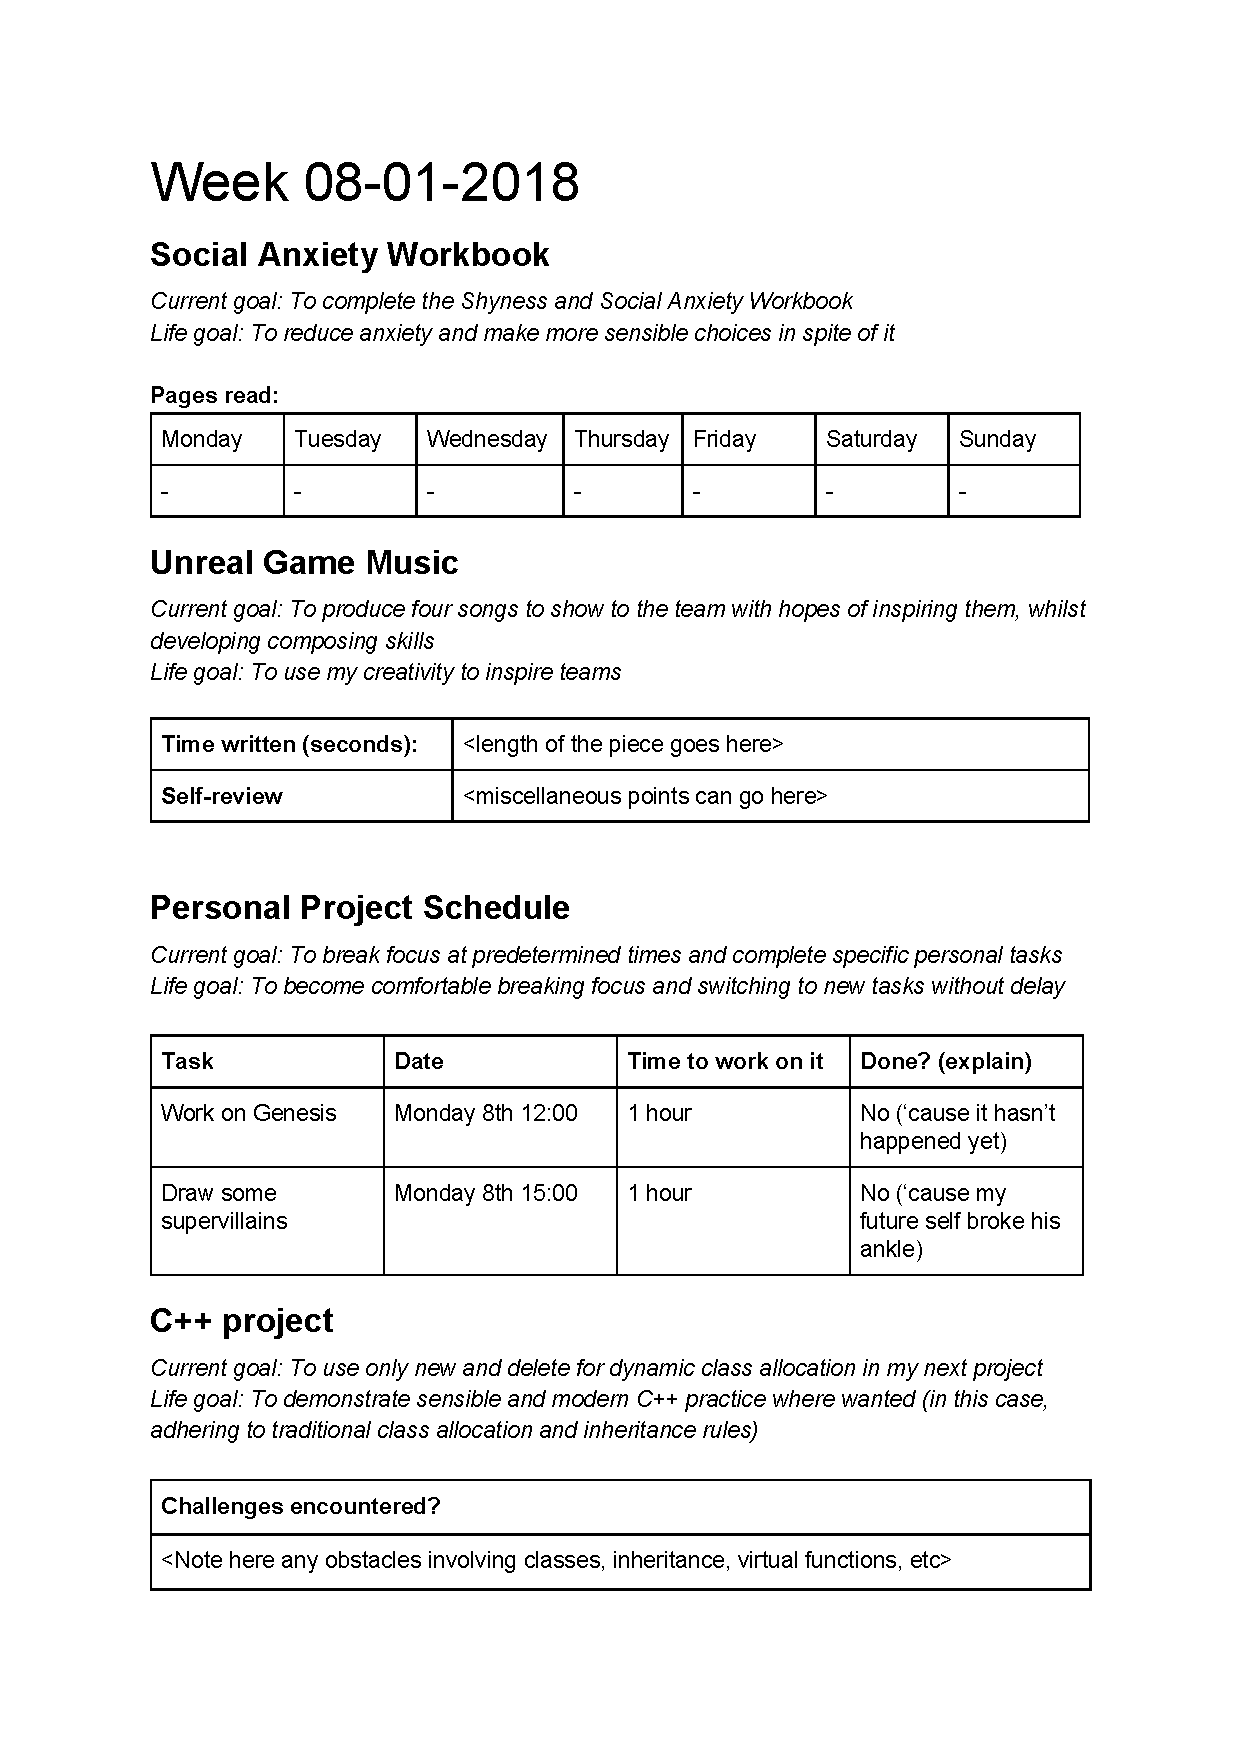
\includegraphics[width=0.7\linewidth]{diary.pdf}}
\caption{Provisional CPD diary template}
\end{figure}

\end{document}
